\documentclass[10pt]{beamer}

\usetheme[progressbar=frametitle]{metropolis}
\usepackage{appendixnumberbeamer}

\usepackage{booktabs}
\usepackage[scale=2]{ccicons}

\usepackage{pgfplots}
\usepgfplotslibrary{dateplot}

\usepackage{graphicx}
\usepackage{caption}
\usepackage{subcaption}
\usepackage{amssymb}
\usepackage{graphicx}
\usepackage{caption}
\usepackage{subcaption}
\usepackage{amsmath}
\usepackage{mathtools}
\usepackage{xspace}
\newcommand{\themename}{\textbf{\textsc{metropolis}}\xspace}

\title{Graph Mining with Edge Uncertainty}
\subtitle{Shortest Path and Centrality Measures}
\date{April 26, 2017}
\author{\textbf{Chi Zhang and Chang Liu}}
%\institute{University of Alberta, Computing Science}
% \titlegraphic{\hfill\includegraphics[height=1.5cm]{logo.pdf}}


\begin{document}
\setbeamercolor{background canvas}{bg=white}
\maketitle

\begin{frame}{Overview}
  \setbeamertemplate{section in toc}[sections numbered]
  \vspace{0.1in}
  \tableofcontents
\end{frame}

\section{Introduction}
\subsection{Background}
\begin{frame}[fragile]{Background}

%  The \themename theme is a Beamer theme with minimal visual noise
%  inspired by the \href{https://github.com/hsrmbeamertheme/hsrmbeamertheme}{\textsc{hsrm} Beamer
%  Theme} by Benjamin Weiss.

%  Enable the theme by loading

 % \begin{verbatim}    \documentclass{beamer}
 %   \usetheme{metropolis}\end{verbatim}

%  Note, that you have to have Mozilla's \emph{Fira Sans} font and XeTeX
 % installed to enjoy this wonderful typography.

In graph theory, \textbf{centrality} identifies the importance of vertices within a graph.
%, which is depicted by \textbf{shortest path}
\vspace{-0.11in}
\begin{figure}[H]
\centering
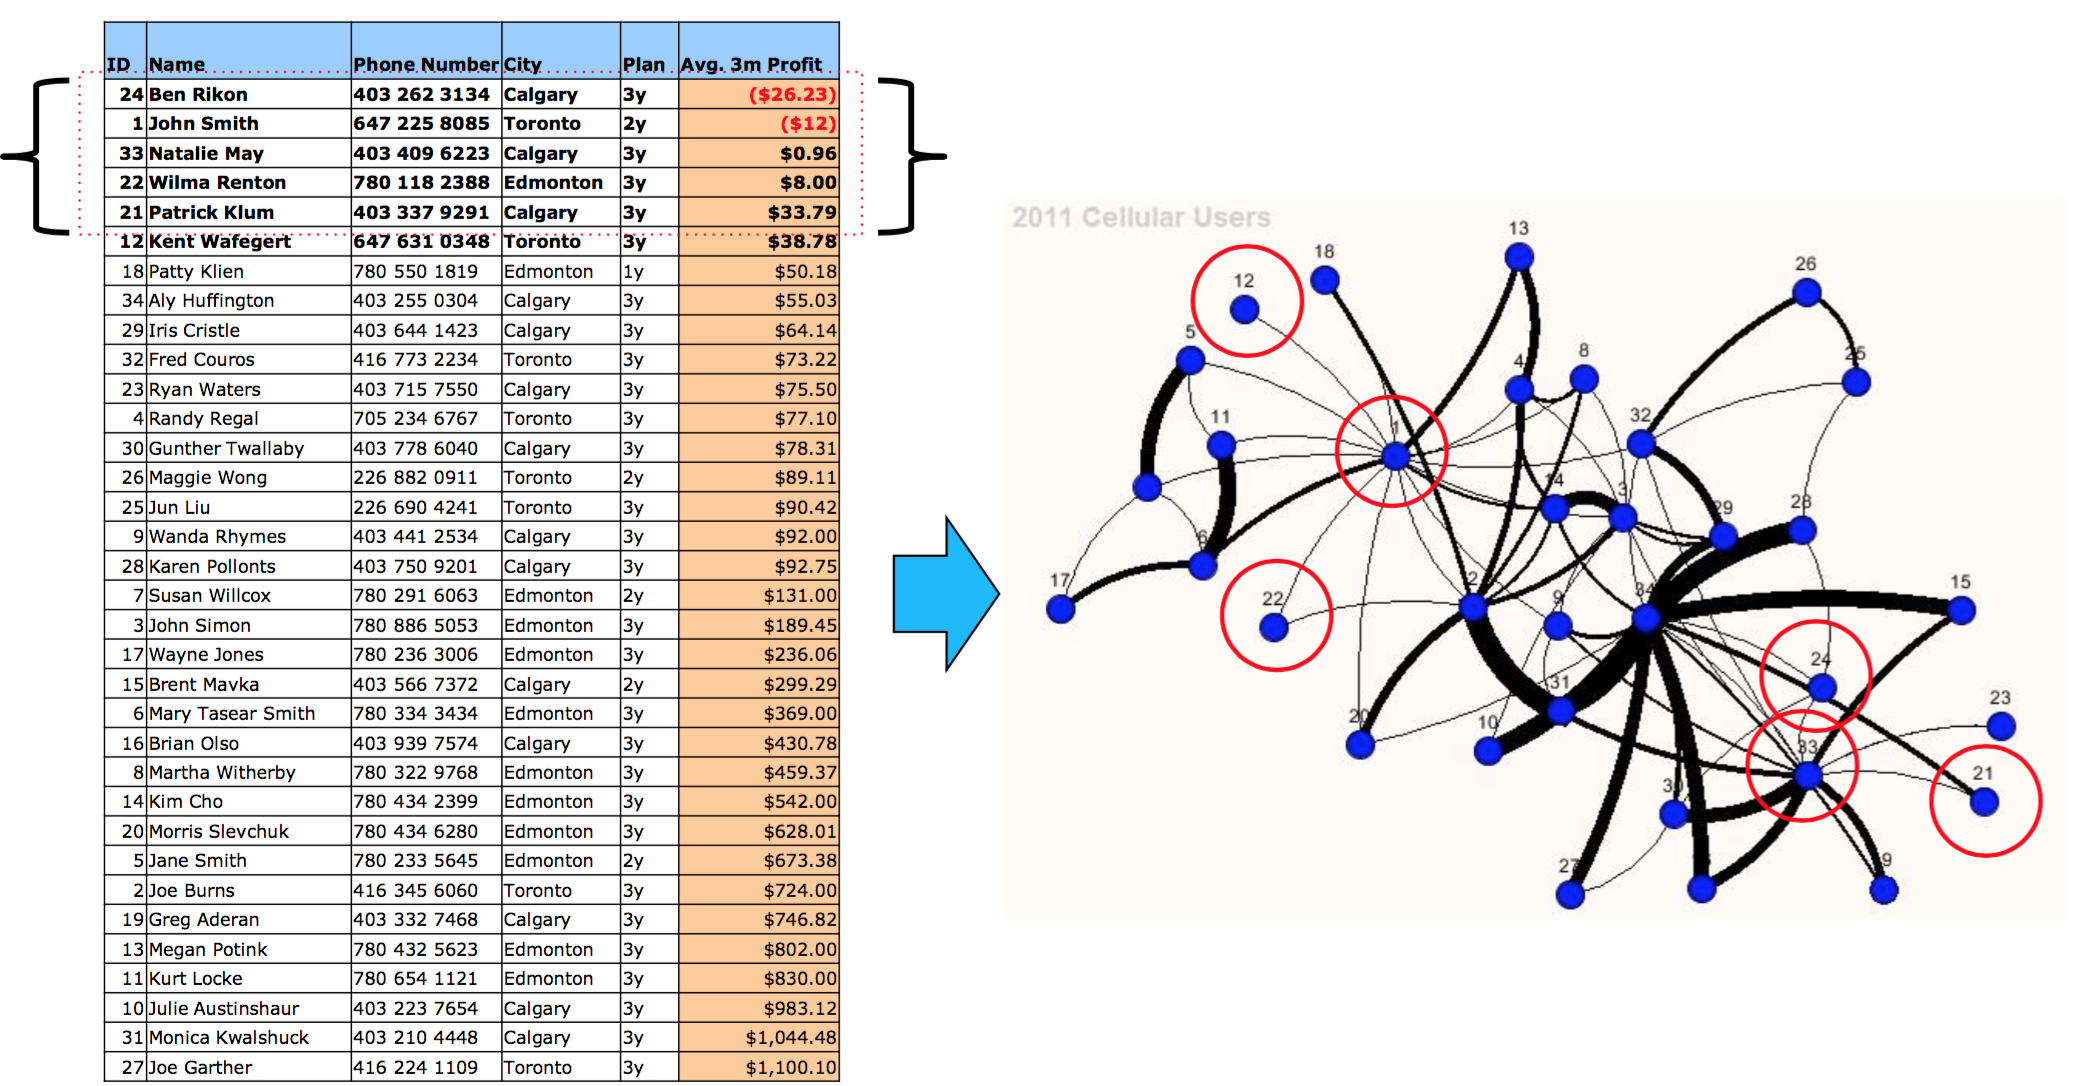
\includegraphics[scale = 0.29]{famous_example.png}
\caption{An example illustrating identifying the most influential person in a social network via centrality}
%\label{famous_example}
\end{figure}
\end{frame}

\begin{frame}
\frametitle{Background: Centrality}

\textbf{Betweenness Centrality}: Measures how many times a node n occurs in a shortest path between any other 2 nodes in the graph;

\textbf{Closeness Centrality}: Mean shortest path distance between a node n and all other nodes reacheable from it;

\end{frame}

%\begin{frame}

%\begin{frame}
%\frametitle{Background: Betweenness Centrality [Wikipedia]}

%The \textbf{betweenness centrality} of a vertex $v$ in a graph $G:=(V,E)$ with $V$ vertices is computed as follows:
%\begin{itemize}
%\item For each pair of vertices $(i,j)$, compute all the \textbf{shortest paths} between them
%\item For each pair of vertices $(i,j)$, determine the \textbf{fraction of shortest paths} that pass through the vertex in question (here, vertex $v$)
%\item Sum this fraction over all pairs of vertices $(i,j)$
%\begin{equation*}
%C_B(v) = \sum_{i\neq v \neq j \in V}\frac{\sigma_{ij}(v)}{\sigma_{ij}}
%\end{equation*}
%\begin{itemize}
%\item $\sigma_{ij}$ is the total number of shortest paths from node $i$ to node $j$ and $\sigma_{ij}(v)$ is the number of those paths that pass through $v$
%\end{itemize}

%\end{itemize}


%\end{frame}

%\begin{frame}
%\frametitle{Background: Closeness Centrality [Wikipedia]}
%   Sections group slides of the same topic

%   \begin{verbatim}    \section{Elements}\end{verbatim}

%   for which \themename provides a nice progress indicator \ldots

%In a connected graph, the \textbf{closeness centrality} of a node is the average length of the \textbf{shortest path} between the node and all other nodes in the graph. Thus the more central a node is, the closer it is to all other nodes.
%\begin{equation*}
%C_C(i) = \frac{1}{\sum_{j}d_{ij}}
%\end{equation*}
%\begin{itemize}
%\item $d_{ij}$ is the \textbf{shortest distance} between vertices $i$ and $j$
%\end{itemize}

%\end{frame}

\subsection{Motivation}
\begin{frame}
\frametitle{Motivation: Uncertainty}
\begin{itemize}
\item Traditional graph centrality measures are applied to discrete, static graphs, where binary edges represent the "presence" or "absence" of a relationship
\item In practice, however, edge uncertainty arises almost everywhere:
\vspace{-0.2in}
\begin{itemize}
\item When considering the evolution of networks overtime, there is inherent uncertainty about the strength of underlying relationships at a particular point in time
\item Even in static graphs, it is sometimes uncertain whether the interaction between two nodes is existed, eg. protein-protein interaction network, crime evidence network, etc.
\end{itemize}
\end{itemize}
\end{frame}

\begin{frame}
\frametitle{Motivation: Probabilistic Graph}
\begin{figure}[H]
\centering
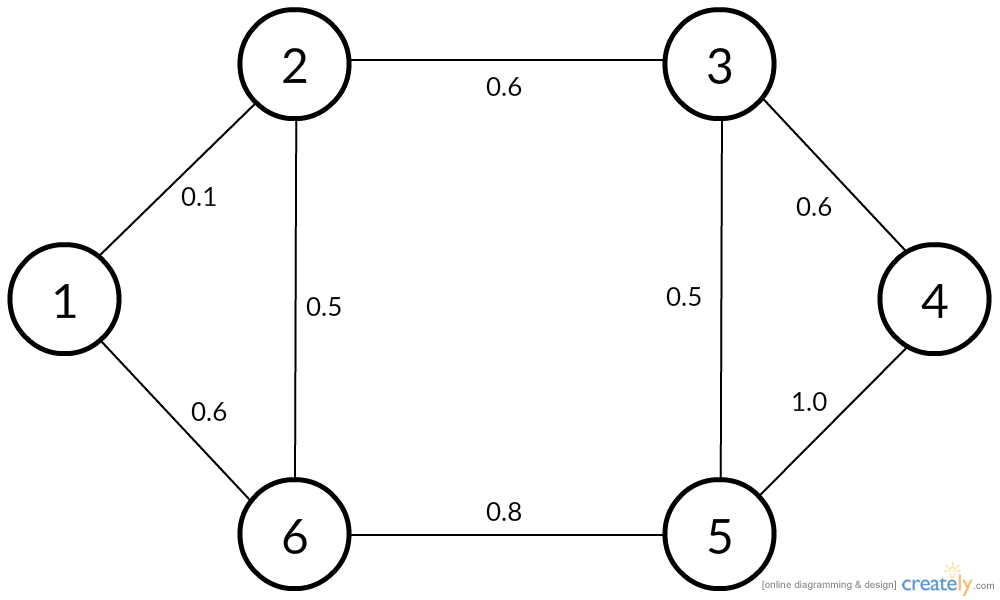
\includegraphics[scale = 0.2]{probabilistic_graph.png}
\caption{An example of probabilistic graph}
%\label{probabilistic_graph}
\end{figure}
\vspace{-0.28in}
This leads to the question that we are looking at: \textbf{Given a probabilistic graph $G := (V,E,P,W)$, where $V$ is a set of vertices, $P$ is the probability distribution over edges $E$, $W$ is the edge attributes, usually weight, how do we compute centrality measures with the presence of edge uncertainty?}
\end{frame}

\section{Related Work}
\subsection{Negative Logarithm \cite{potamias2009nearest}}
\begin{frame}{Negative Logarithm \cite{potamias2009nearest}}
% 	\themename supports 4 different titleformats:
% 	\begin{itemize}
% 		\item Regular
% 		\item \textsc{Smallcaps}
% 		\item \textsc{allsmallcaps}
% 		\item ALLCAPS
% 	\end{itemize}
% 	They can either be set at once for every title type or individually.
\begin{itemize}
\item A simple approach is to consider the probabilities
as costs by taking the negative logarithm of the probability; the weight between two adjacent vertices $i$ and $j$ are defined as follow:
\begin{equation*}
W(e_{uv}) = -log(P(e_{uv}))
\end{equation*}
\vspace{-0.2in}
\begin{itemize}
\item $P(e_{uv})$ is the probability defined on edge $e_{uv}$
\item $W(e_{uv})$ is the new weight defined by the negative logarithm of edge probability
\end{itemize}
\item Thus probabilities are converted to weights and all existential graph mining methods on discrete graphs become accessible under this framework
\end{itemize}
\end{frame}

% {
%     \metroset{titleformat frame=smallcaps}
% \begin{frame}{Small caps}
% 	This frame uses the \texttt{smallcaps} titleformat.

% 	\begin{alertblock}{Potential Problems}
% 		Be aware, that not every font supports small caps. If for example you typeset your presentation with pdfTeX and the Computer Modern Sans Serif font, every text in smallcaps will be typeset with the Computer Modern Serif font instead.
% 	\end{alertblock}
% \end{frame}
% }
\subsection{Most Probable Path \cite{pfeiffer2010probabilistic}, \cite{pfeiffer2011methods}}
\begin{frame}{Most Probable Path \cite{pfeiffer2010probabilistic}, \cite{pfeiffer2011methods}}
\begin{itemize}
\item Using the notion of probabilistic paths, we calculate the probability of the existence of a path $\rho_{ij}$ between nodes $i$ and $j$ as follows:
\begin{equation*}
P(\rho_{ij}) = \prod_{e_{uv} \in E}P(e_{uv})
\end{equation*}
\vspace{-0.12in}
\begin{itemize}
\item $e_{uv}$ is the edge connecting two adjacent nodes $u$ and $v$
\end{itemize}
\item Now given two nodes $i$ and $j$, the \textbf{most probable path} is simply the one with \textit{maximum likelihood}:
\[ \rho_{ij}^{ML} = argmaxP(\rho_{ij}) \]
\item Then we can compute the most probable path by applying Dijkstra's shortest path algorithm, but expanding on the most probable path instead
\end{itemize}
\end{frame}

% {
% \metroset{titleformat frame=allsmallcaps}
% \begin{frame}{All small caps}
% 	This frame uses the \texttt{allsmallcaps} titleformat.

% 	\begin{alertblock}{Potential problems}
% 		As this titleformat also uses smallcaps you face the same problems as with the \texttt{smallcaps} titleformat. Additionally this format can cause some other problems. Please refer to the documentation if you consider using it.

% 		As a rule of thumb: Just use it for plaintext-only titles.
% 	\end{alertblock}
% \end{frame}
% }

% {
% \metroset{titleformat frame=allcaps}
% \begin{frame}{All caps}
% 	This frame uses the \texttt{allcaps} titleformat.

% 	\begin{alertblock}{Potential Problems}
% 		This titleformat is not as problematic as the \texttt{allsmallcaps} format, but basically suffers from the same deficiencies. So please have a look at the documentation if you want to use it.
% 	\end{alertblock}
% \end{frame}
% }

\section{Our Approach}
\begin{frame}[fragile]{Inversed Probabilistic Graph}
%       \begin{verbatim}The theme provides sensible defaults to
% \emph{emphasize} text, \alert{accent} parts
% or show \textbf{bold} results.\end{verbatim}

%   \begin{center}becomes\end{center}

%   The theme provides sensible defaults to \emph{emphasize} text,
%   \alert{accent} parts or show \textbf{bold} results.

To circumvent the relatively heavy computation of \textit{Most Probable Path} method and the low accuracy of \textit{Negative Logarithm} method, we propose a new approach, \textbf{Inversed Probabilistic Graph}, defined as follows:
\begin{itemize}
\item Given a probabilistic graph $G:=(V,E,P,W)$, for an edge $e_{uv}$, we can convert probability to weight by taking the inverse of edge probability
\[ W'(e_{uv}) = \frac{W(e_{uv})}{P(e_{uv})^\lambda }\]
\vspace{-0.15in}
\begin{itemize}
\item Here $\lambda$ is a hyper-parameter, $W'$ is the newly computed weight for an edge
\item In experiment we use $\lambda = 0.4$
\end{itemize}
\end{itemize}
Again, we can apply existential graph mining algorithms under this framework
\end{frame}

\section{Experiment Results}


\begin{frame}
\frametitle{Illustrative Experiment}
\begin{itemize}
\item Firstly, we draw two graphs, each demonstrating the centrality ranking evolution of selected individuals in the Enron dataset, as \textit{Pfeiffer et al} did in \cite{pfeiffer2010probabilistic}, \cite{pfeiffer2011methods}

\item We evaluate our method by looking at each graph if centrality evolutions correspond to the background provided in the Enron dataset


\end{itemize}
\end{frame}

\begin{frame}
\frametitle{Centrality Ranking over Time in Enron: Lay and Skilling}
\begin{figure}[H]
\centering
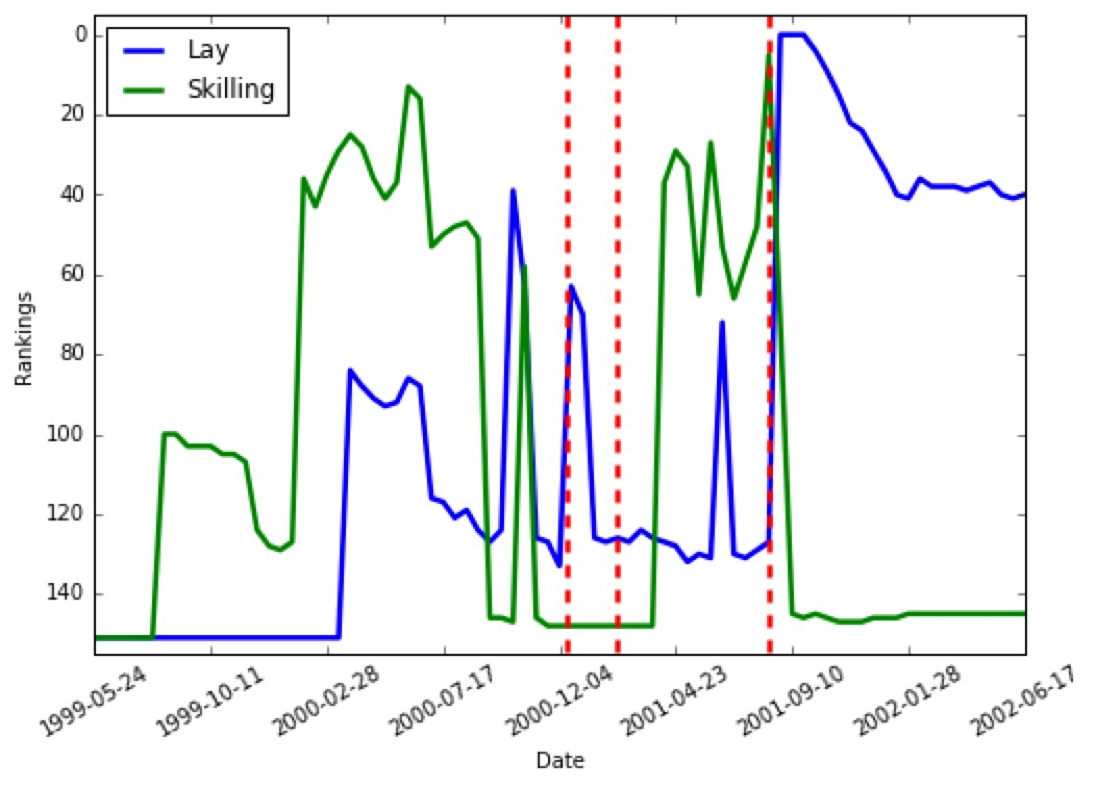
\includegraphics[scale = 0.3]{rank_change1.png}
\caption{Centrality ranking evolution of Lay and Skilling}
%\label{probabilistic_graph}
\end{figure}
\vspace{-0.15in}
\begin{itemize}
\item On December $13^{th}$, 2000, it was announced that Skilling would assume the CEO position at Enron, with Lay retiring but remaining as a chairman.
\item During February 2001, Skilling made the transition to CEO and Lay retired
\item On August $14^{th}$, 2001, Skilling resigned from the position of CEO and Lay took over
\end{itemize}
\end{frame}


\begin{frame}
\frametitle{Centrality Ranking over Time in Enron: Kitchen and Lavorato}
\begin{figure}[H]
\centering
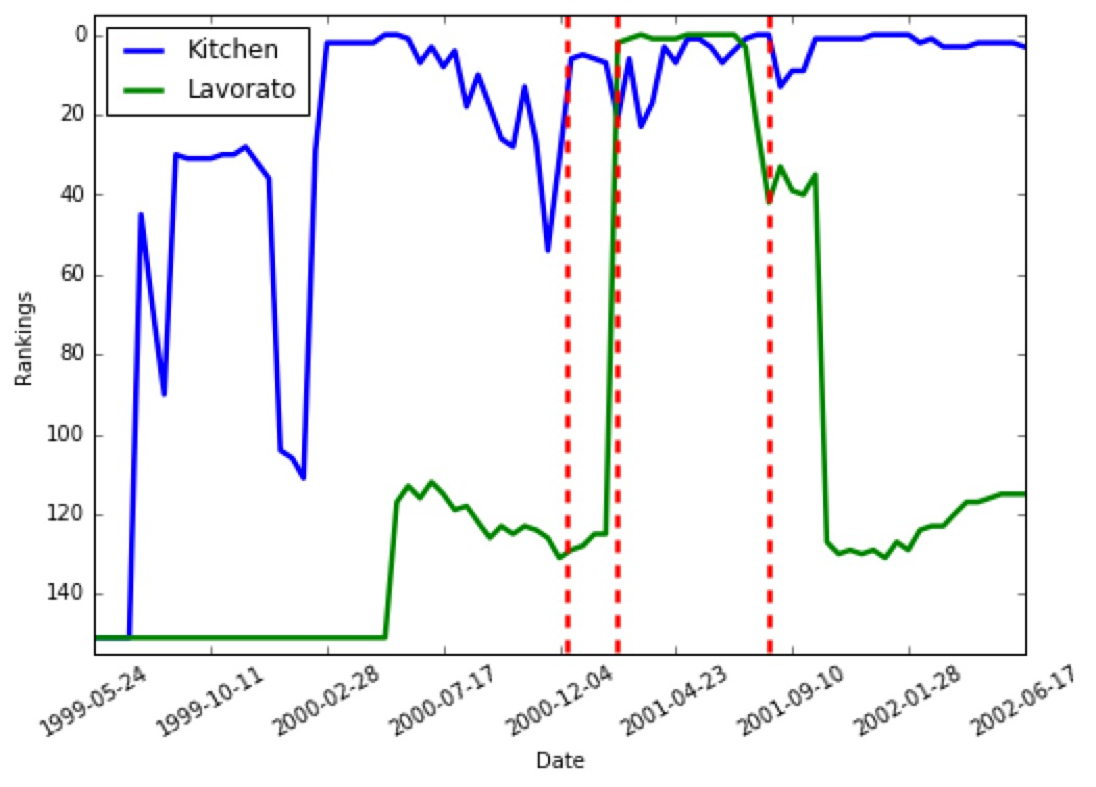
\includegraphics[scale = 0.3]{rank_change2.png}
\caption{Centrality ranking evolution of Kitchen and Lavorato}
%\label{probabilistic_graph}
\end{figure}
\vspace{-0.15in}
\begin{itemize}
\item Kitchen and Lavorato were executives for Enron Americas
\item Lavorato is only important during Skilling's tenure as CEO; his centrality drops noticeably otherwise. This suggests that Skilling and Lavorato were extremely close
\item On the other hand, Kitchen had extremely high rankings throughout
\end{itemize}
\end{frame}

\begin{frame}
\frametitle{Comparative Experiment}
\begin{itemize}
\item Secondly, we compare the two methods, \textit{Negative Logarithm} and \textit{Most Probable Path} that are illustrated above, with our method on 
\begin{itemize}
\item Enron dataset
\item Simulated weighted graph dataset and discrete unweighted graph dataset
\end{itemize}
\item We evaluate each method via visualizing the linear relationship between centrality rankings computed by each method and average centrality rankings computed by sampling
\item The stronger linear relationship that a plot indicates, the better performance the method is.
\item The metric of the linear relationship strength:
\[ r=\frac{\sum_{i=1}^{m}|x_i-y_i|}{\sqrt{2}m} \]
\end{itemize}
\end{frame}



\begin{frame}
\frametitle{Centralities on Enron Dataset}
\vspace{0.15in}
\begin{figure}[H]
\centering
\begin{subfigure}{.32\textwidth}
  \centering
  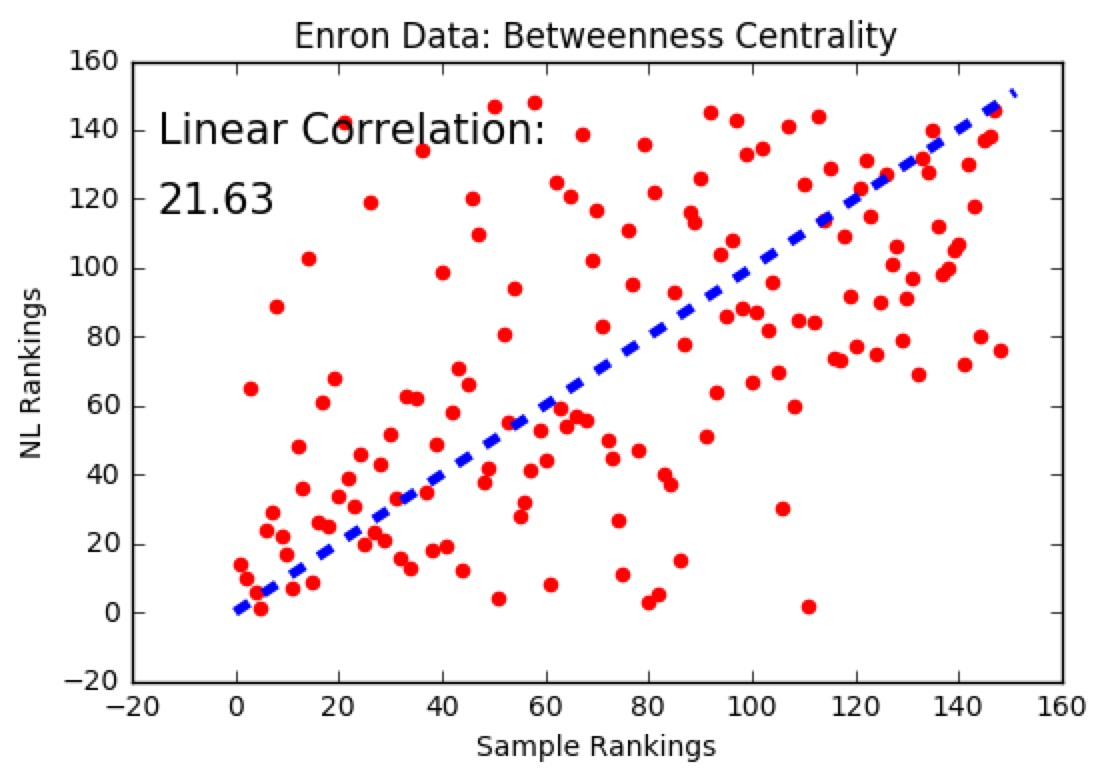
\includegraphics[width=0.95\linewidth]{EBC_NL.jpeg}
%  \caption{Per-map suboptimality}
%  \label{acpermap}
\end{subfigure}
%\caption{Normalized mean suboptimality on the per-map and uni-map bases for GBDT, SVM, and NN classifiers using AlexNet as a feature extractor}
\begin{subfigure}{.32\textwidth}
	\centering
    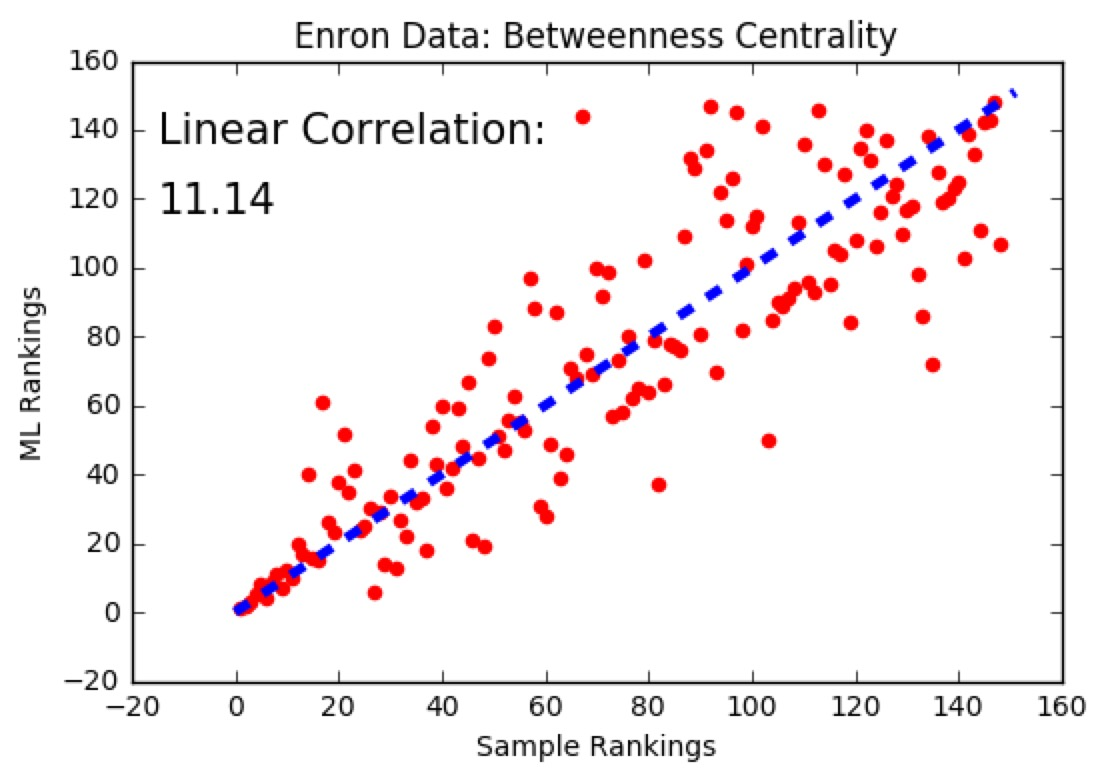
\includegraphics[width=0.95\linewidth]{EBC_ML.jpeg}
\end{subfigure}
%\label{alexclass}
\begin{subfigure}{.32\textwidth}
	\centering
    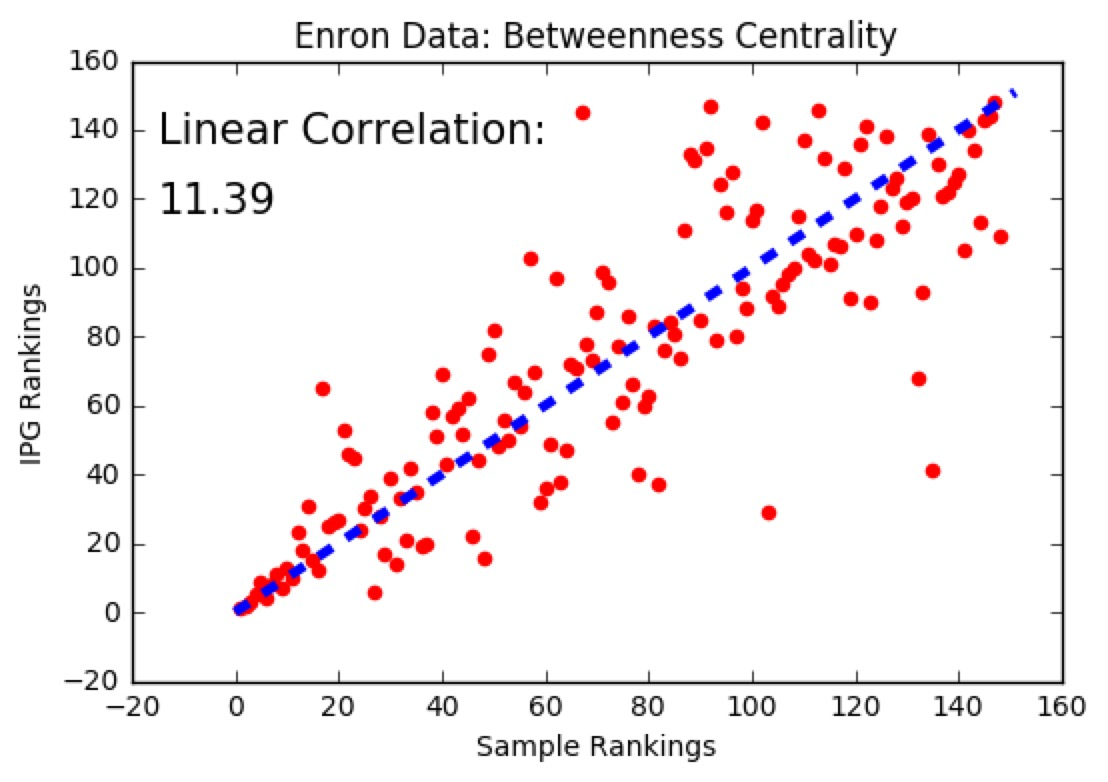
\includegraphics[width=0.95\linewidth]{EBC_IPG.jpeg}
\end{subfigure}
\caption{Comparison of betweenness centralities computed by different methods on Enron dataset}
\end{figure}
\vspace{-0.1in}
\begin{figure}[H]
\centering
\begin{subfigure}{.32\textwidth}
  \centering
  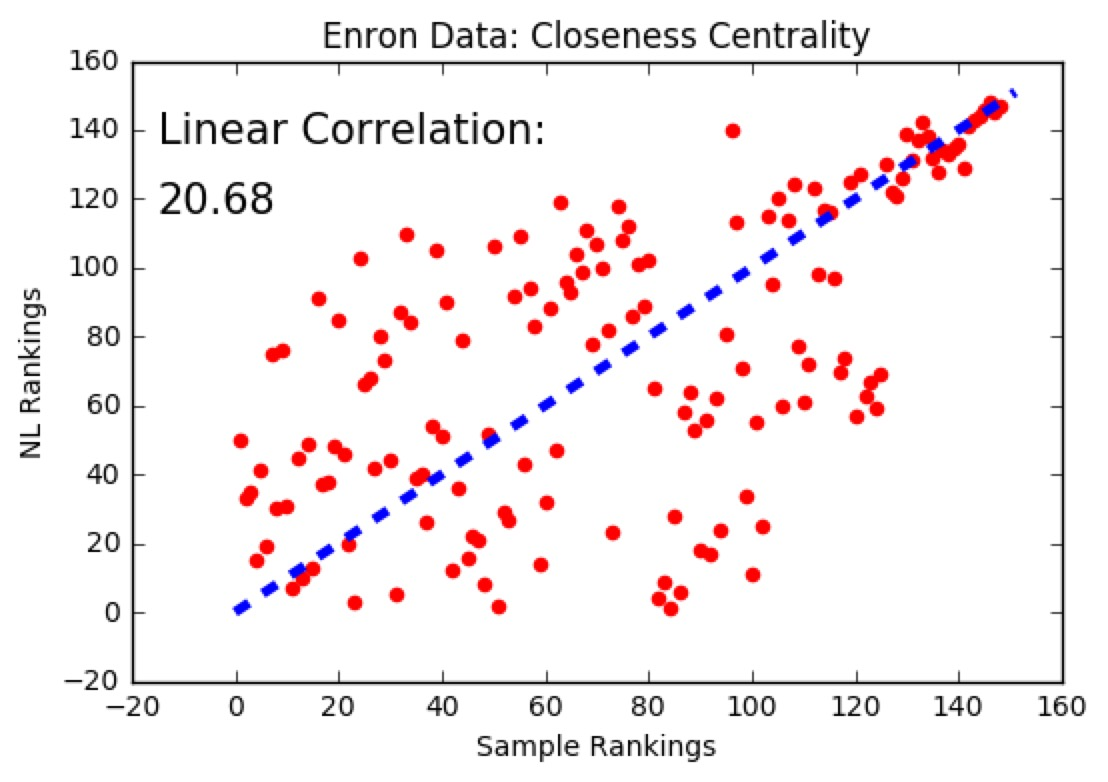
\includegraphics[width=0.95\linewidth]{ECC_NL.jpeg}
%  \caption{Per-map suboptimality}
%  \label{acpermap}
\end{subfigure}
%\caption{Normalized mean suboptimality on the per-map and uni-map bases for GBDT, SVM, and NN classifiers using AlexNet as a feature extractor}
\begin{subfigure}{.32\textwidth}
	\centering
    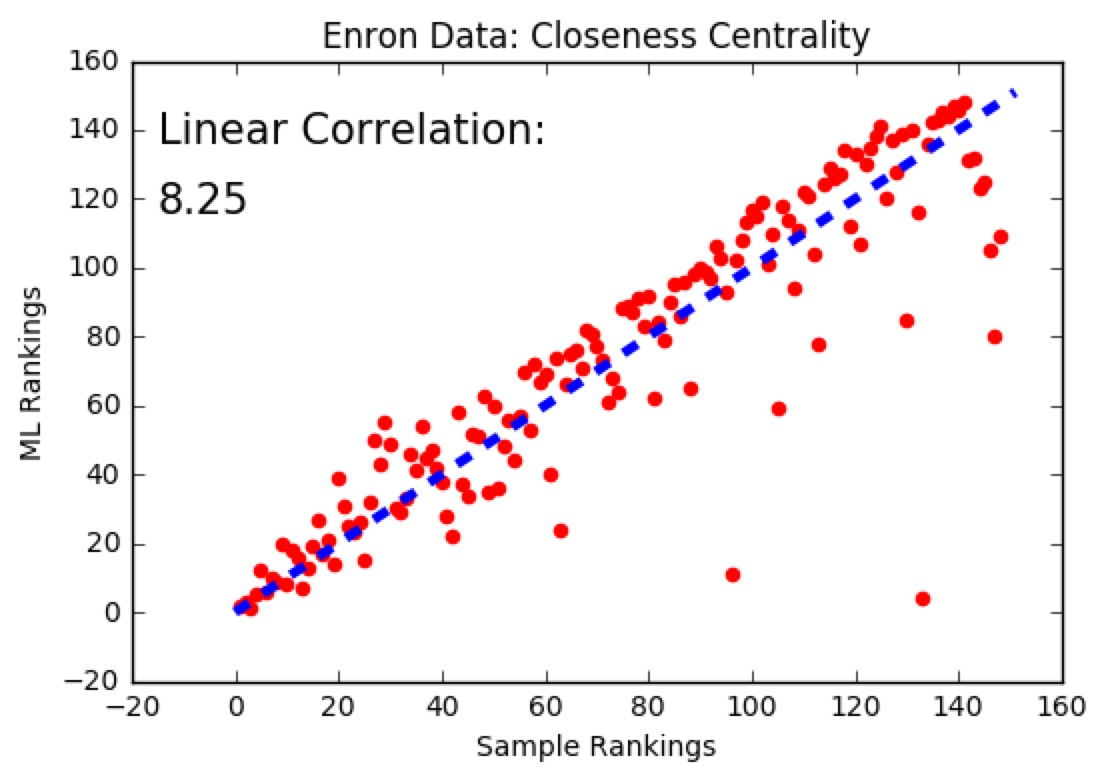
\includegraphics[width=0.95\linewidth]{ECC_ML.jpeg}
\end{subfigure}
%\label{alexclass}
\begin{subfigure}{.32\textwidth}
	\centering
    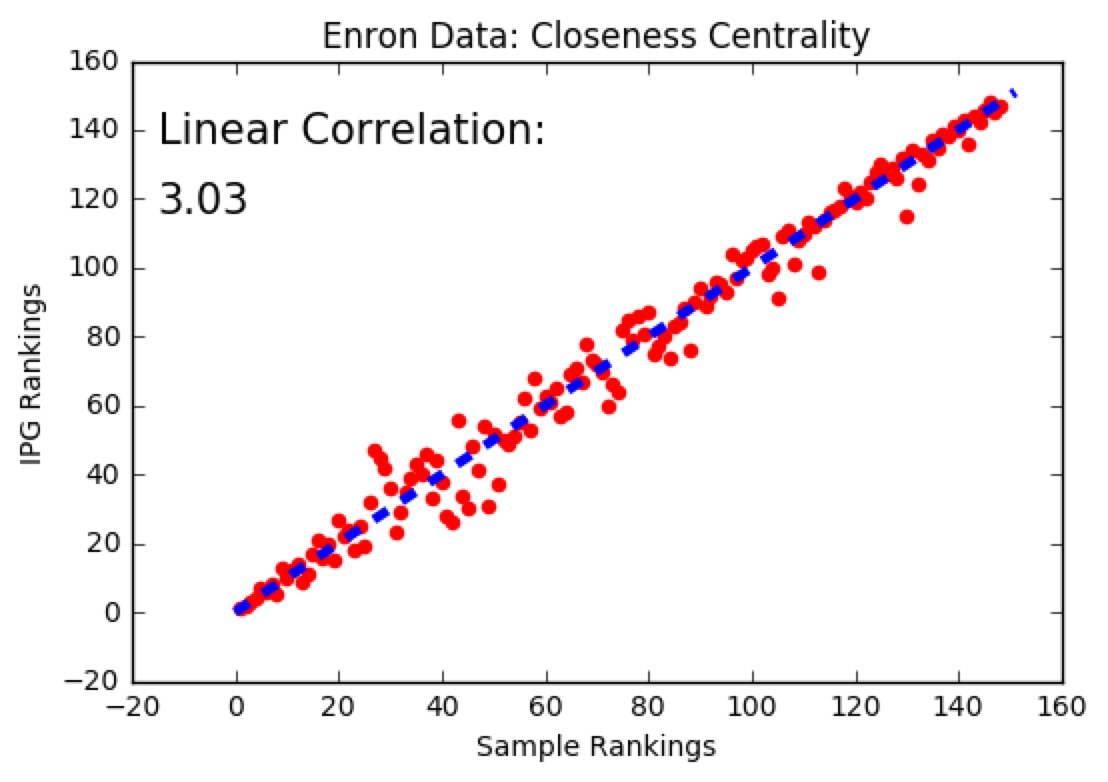
\includegraphics[width=0.95\linewidth]{ECC_IPG.jpeg}
\end{subfigure}
\caption{Comparison of closeness centralities computed by different methods on Enron dataset}
\end{figure}
%\caption{Betweenness Centrality on Enron Dataset}
\end{frame}



\begin{frame}
\frametitle{Centralities on Simulated Unweighted Graphs}
\vspace{0.15in}
\begin{figure}[H]
\centering
\begin{subfigure}{.32\textwidth}
  \centering
  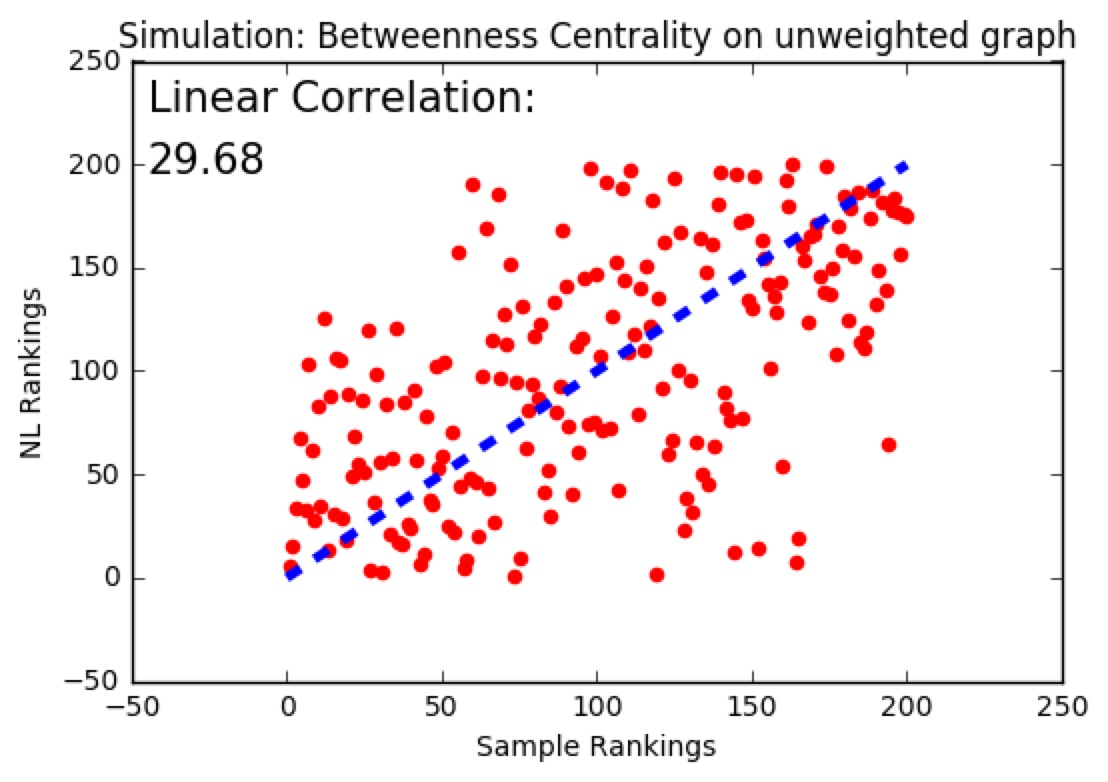
\includegraphics[width=0.95\linewidth]{BCU_NL.jpeg}
%  \caption{Per-map suboptimality}
%  \label{acpermap}
\end{subfigure}
%\caption{Normalized mean suboptimality on the per-map and uni-map bases for GBDT, SVM, and NN classifiers using AlexNet as a feature extractor}
\begin{subfigure}{.32\textwidth}
	\centering
    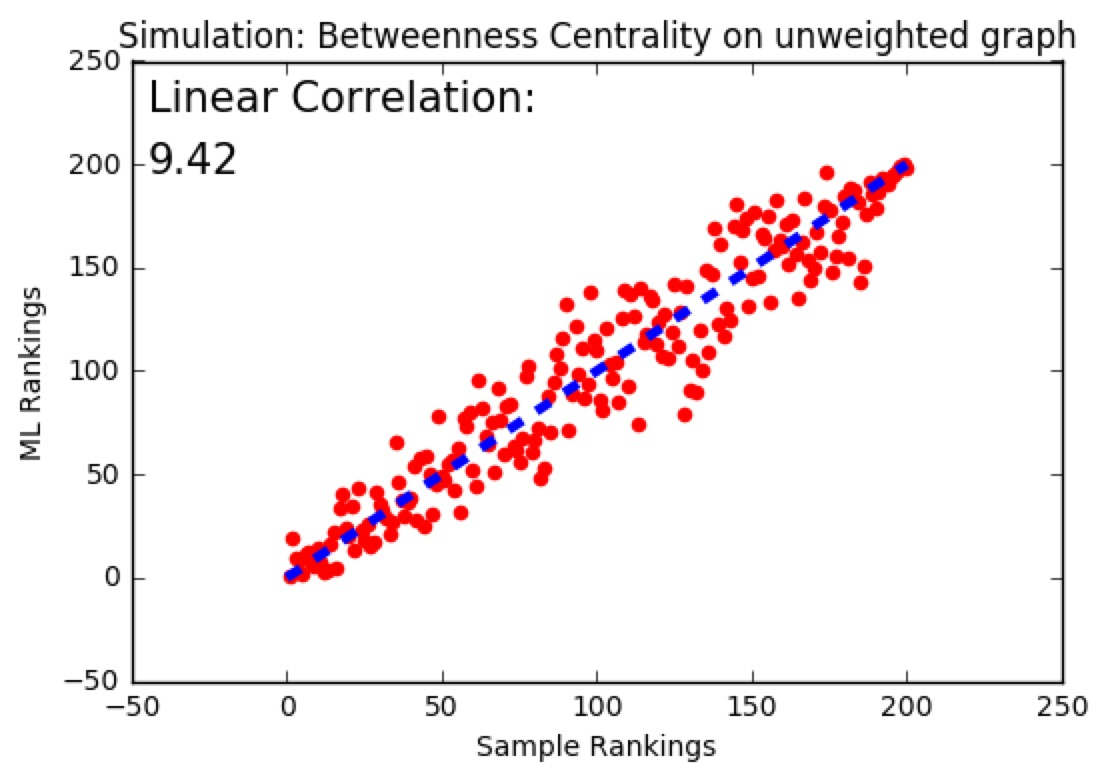
\includegraphics[width=0.95\linewidth]{BCU_ML.jpeg}
\end{subfigure}
%\label{alexclass}
\begin{subfigure}{.32\textwidth}
	\centering
    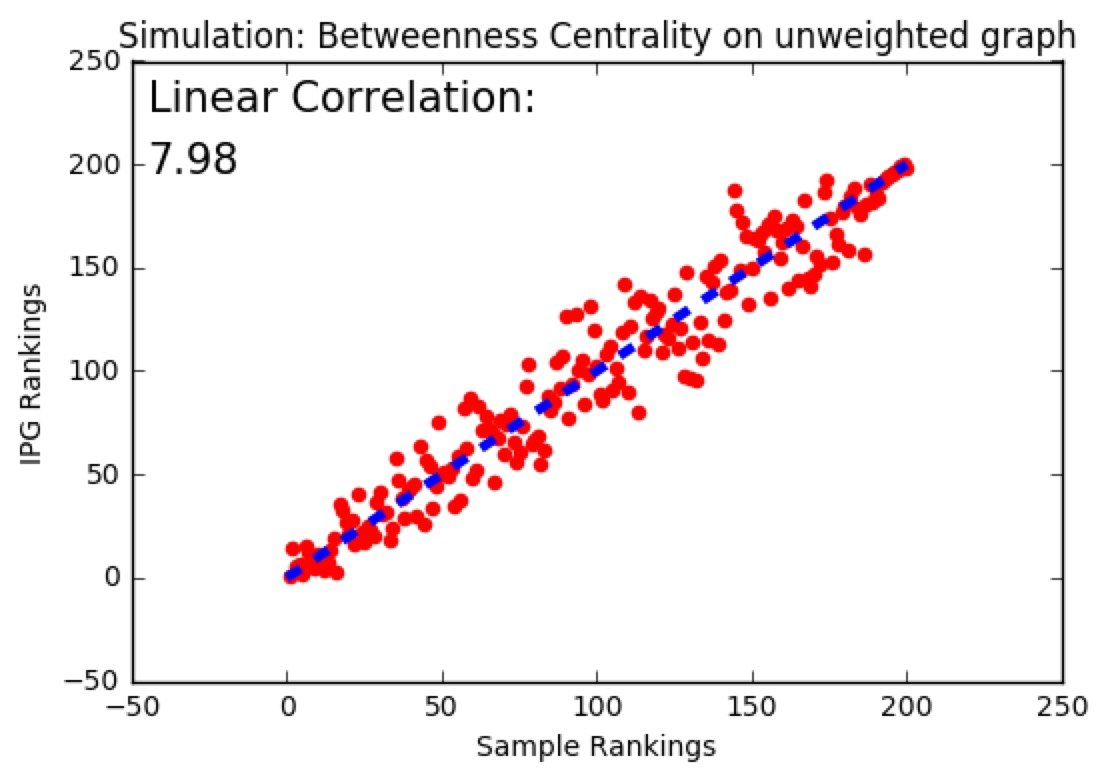
\includegraphics[width=0.95\linewidth]{BCU_IPG.jpeg}
\end{subfigure}
\caption{Comparison of betweenness centralities computed by different methods on simulated unweighted graphs}
\end{figure}
\vspace{-0.1in}
\begin{figure}[H]
\centering
\begin{subfigure}{.32\textwidth}
  \centering
  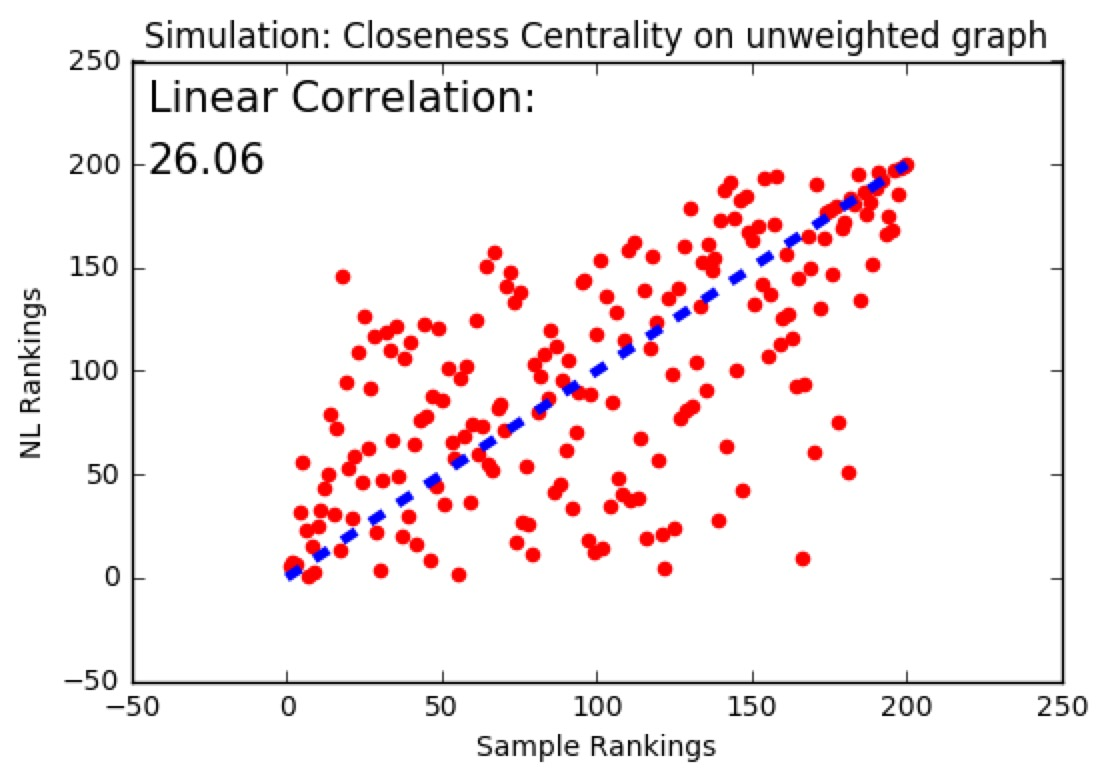
\includegraphics[width=0.95\linewidth]{CCU_NL.jpeg}
%  \caption{Per-map suboptimality}
%  \label{acpermap}
\end{subfigure}
%\caption{Normalized mean suboptimality on the per-map and uni-map bases for GBDT, SVM, and NN classifiers using AlexNet as a feature extractor}
\begin{subfigure}{.32\textwidth}
	\centering
    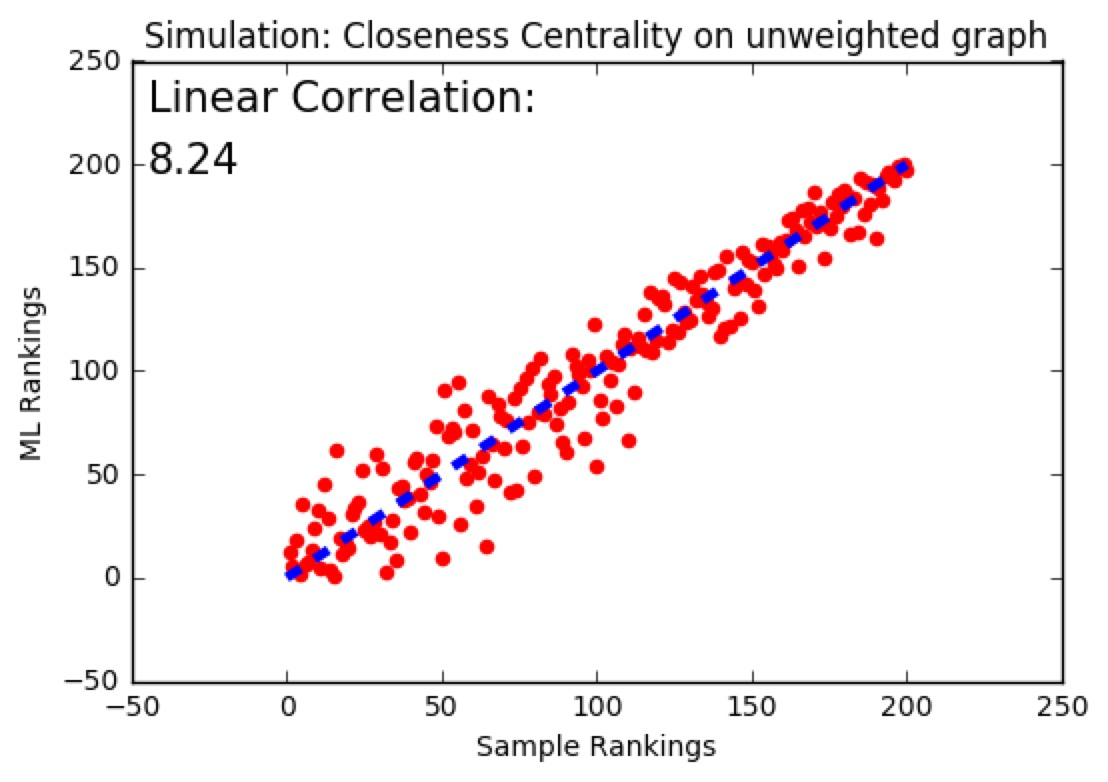
\includegraphics[width=0.95\linewidth]{CCU_ML.jpeg}
\end{subfigure}
%\label{alexclass}
\begin{subfigure}{.32\textwidth}
	\centering
    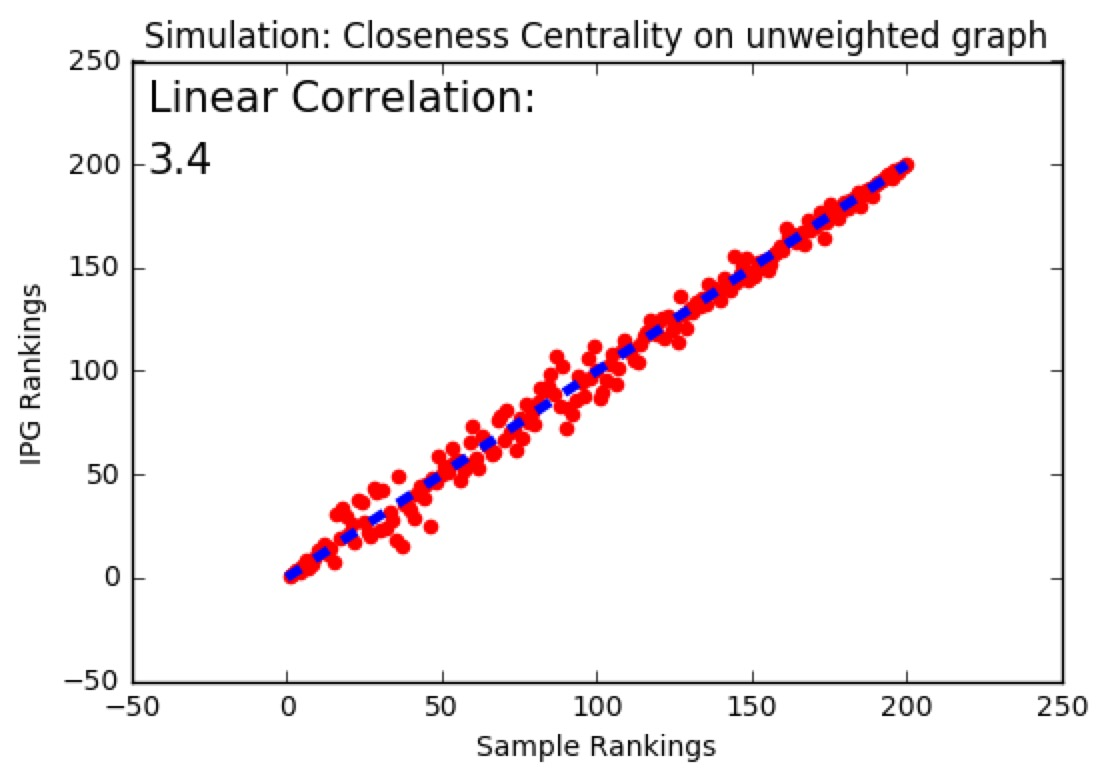
\includegraphics[width=0.95\linewidth]{CCU_IPG.jpeg}
\end{subfigure}
\caption{Comparison of closeness centralities computed by different methods on simulated unweighted graphs}
\end{figure}
%\caption{Betweenness Centrality on Enron Dataset}
\end{frame}


\begin{frame}
\frametitle{Centralities on Simulated Weighted Graphs}
\vspace{0.15in}
\begin{figure}[H]
\centering
\begin{subfigure}{.32\textwidth}
  \centering
  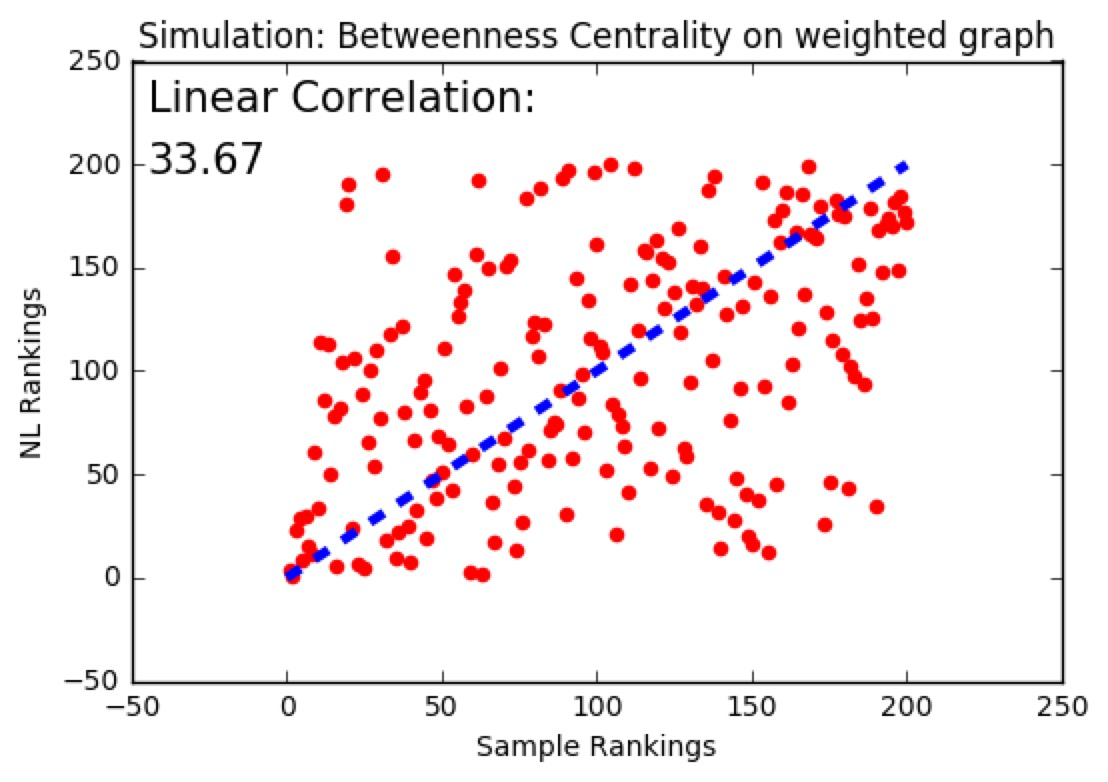
\includegraphics[width=0.95\linewidth]{BCW_NL.jpeg}
%  \caption{Per-map suboptimality}
%  \label{acpermap}
\end{subfigure}
%\caption{Normalized mean suboptimality on the per-map and uni-map bases for GBDT, SVM, and NN classifiers using AlexNet as a feature extractor}
\begin{subfigure}{.32\textwidth}
	\centering
    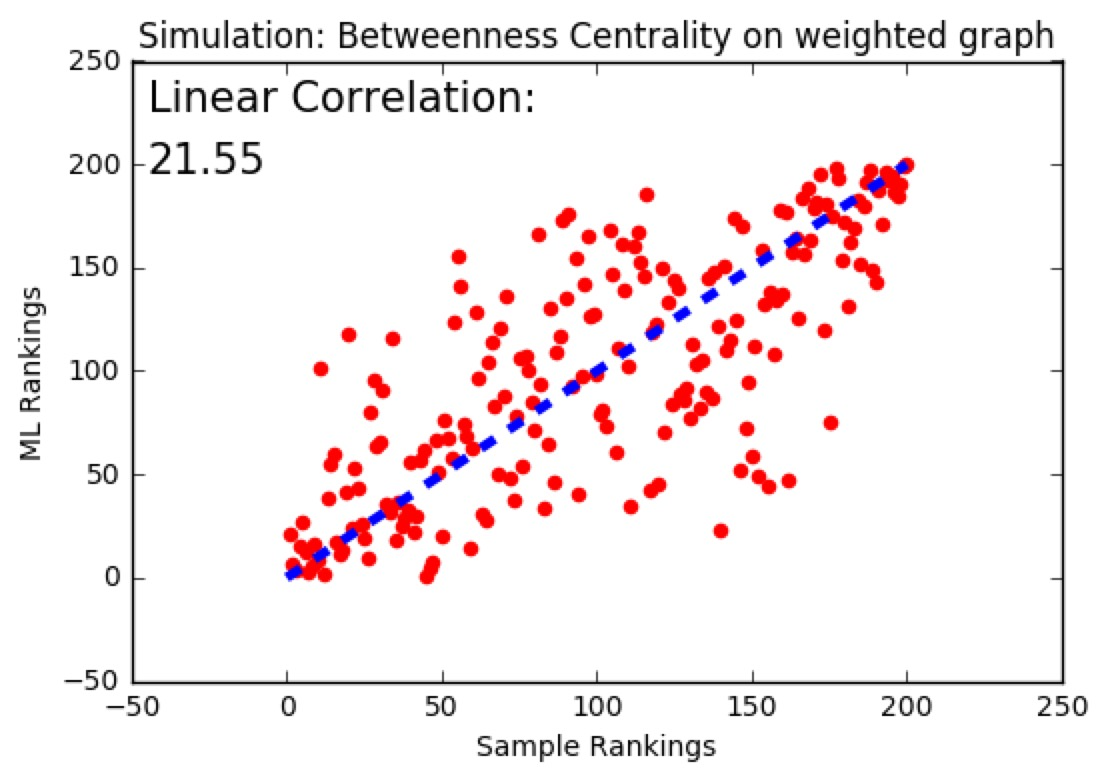
\includegraphics[width=0.95\linewidth]{BCW_ML.jpeg}
\end{subfigure}
%\label{alexclass}
\begin{subfigure}{.32\textwidth}
	\centering
    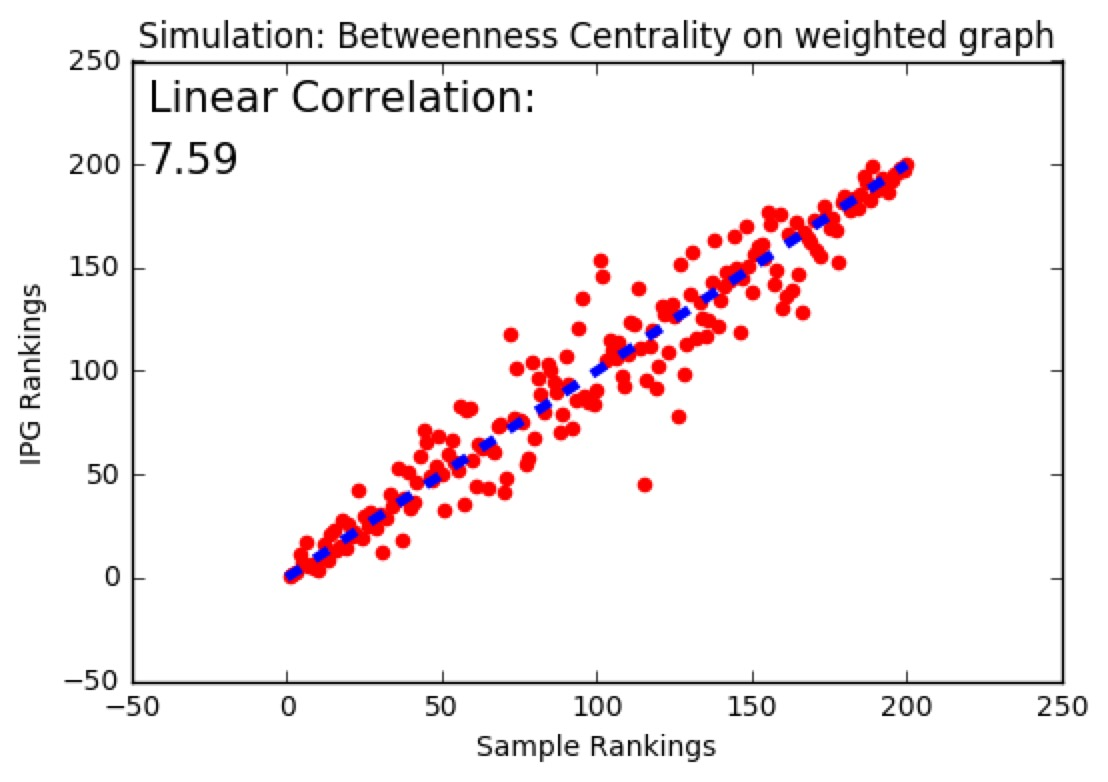
\includegraphics[width=0.95\linewidth]{BCW_IPG.jpeg}
\end{subfigure}
\caption{Comparison of betweenness centralities computed by different methods on simulated weighted graphs}
\end{figure}
\vspace{-0.1in}
\begin{figure}[H]
\centering
\begin{subfigure}{.32\textwidth}
  \centering
  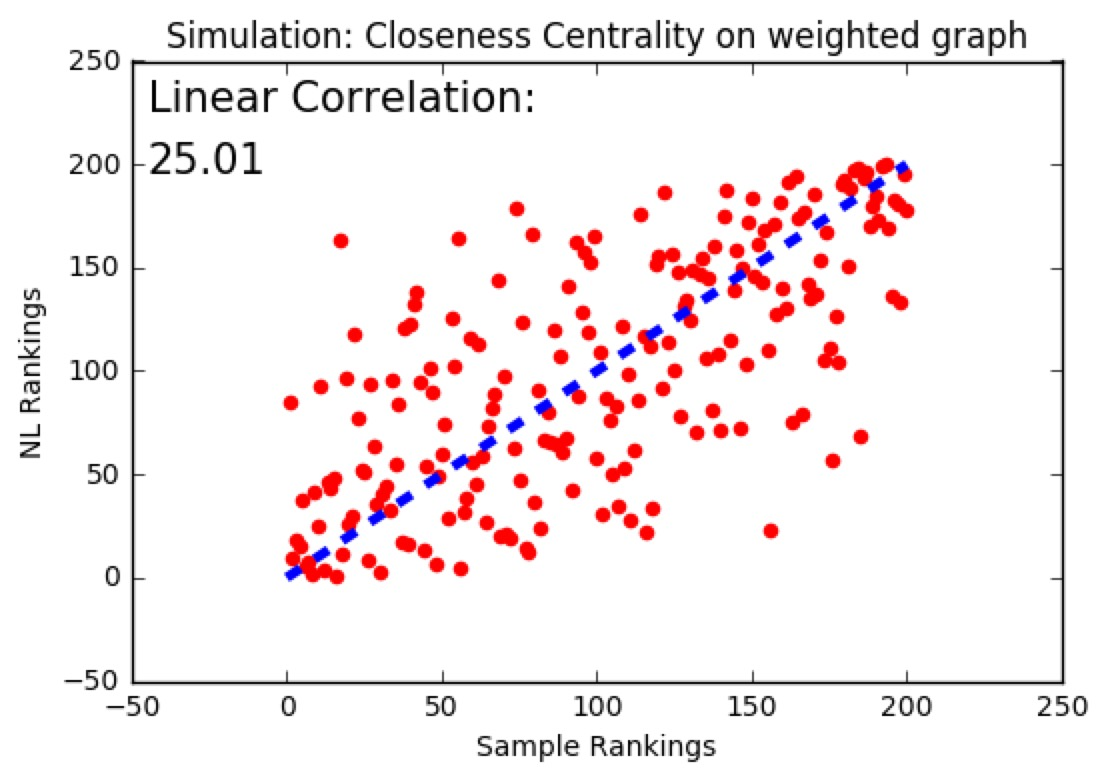
\includegraphics[width=0.95\linewidth]{CCW_NL.jpeg}
%  \caption{Per-map suboptimality}
%  \label{acpermap}
\end{subfigure}
%\caption{Normalized mean suboptimality on the per-map and uni-map bases for GBDT, SVM, and NN classifiers using AlexNet as a feature extractor}
\begin{subfigure}{.32\textwidth}
	\centering
    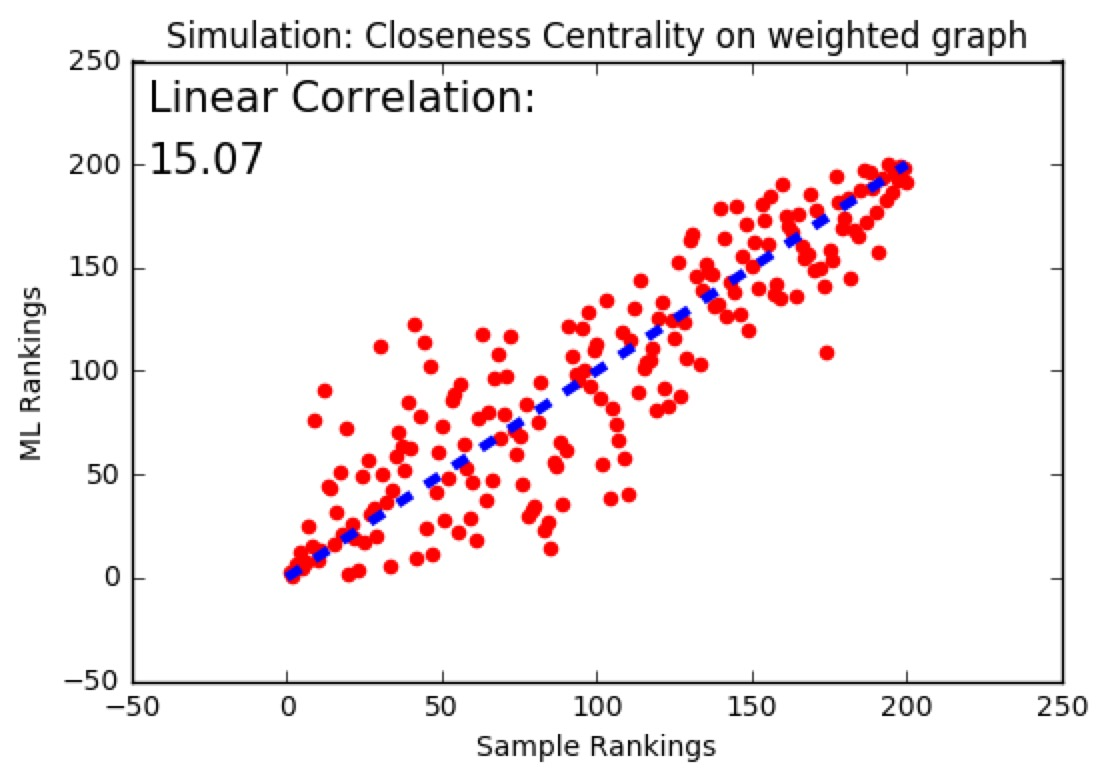
\includegraphics[width=0.95\linewidth]{CCW_ML.jpeg}
\end{subfigure}
%\label{alexclass}
\begin{subfigure}{.32\textwidth}
	\centering
    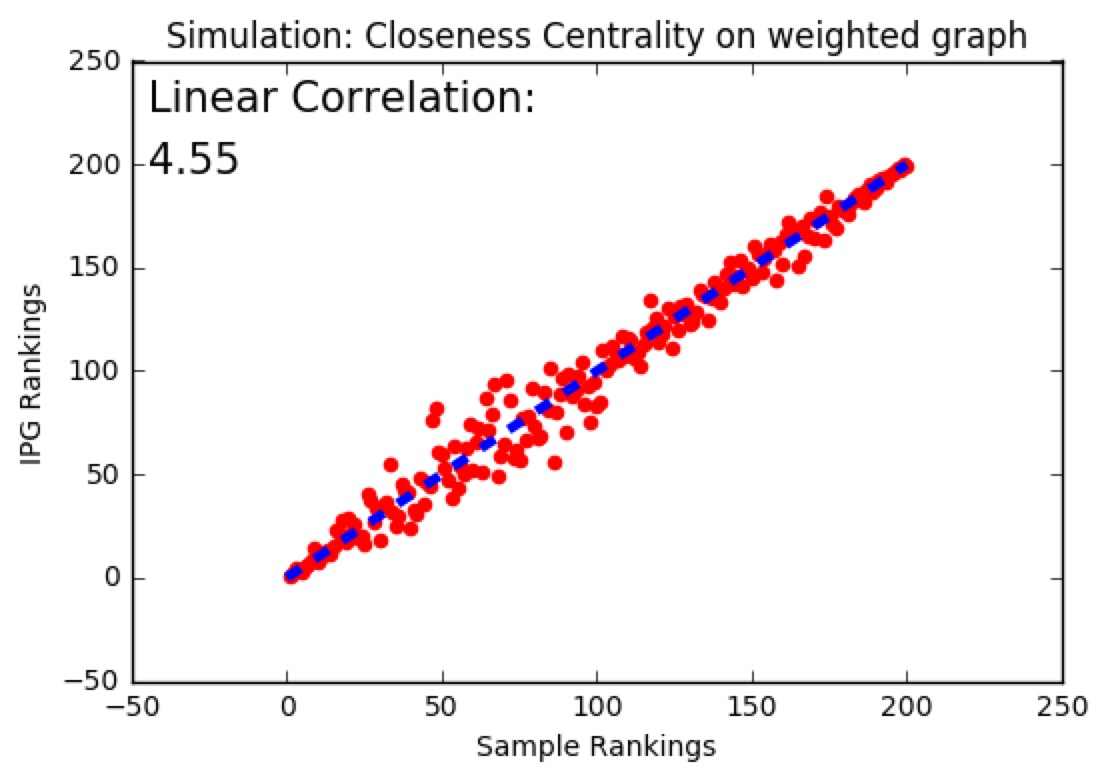
\includegraphics[width=0.95\linewidth]{CCW_IPG.jpeg}
\end{subfigure}
\caption{Comparison of closeness centralities computed by different methods on simulated weighted graphs}
\end{figure}
%\caption{Betweenness Centrality on Enron Dataset}
\end{frame}

\begin{frame}
\frametitle{Application: Link Prediction}
\vspace{0.15in}
\begin{figure}[H]
\centering
\begin{subfigure}{.9\textwidth}
  \centering
  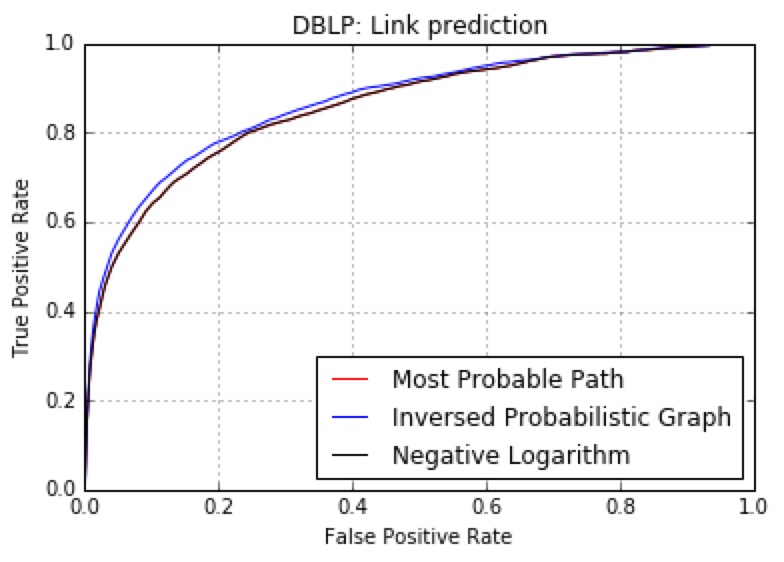
\includegraphics[width=1\linewidth]{LP.jpeg}
%  \caption{Per-map suboptimality}
%  \label{acpermap}
\end{subfigure}

\caption{Link Prediction}
\end{figure}
%\caption{Betweenness Centrality on Enron Dataset}
\end{frame}

\begin{frame}
\frametitle{Selection of Optimal Hyper-parameter $\lambda$}
\vspace{0.15in}
\begin{figure}[H]
\centering
\begin{subfigure}{.4\textwidth}
  \centering
  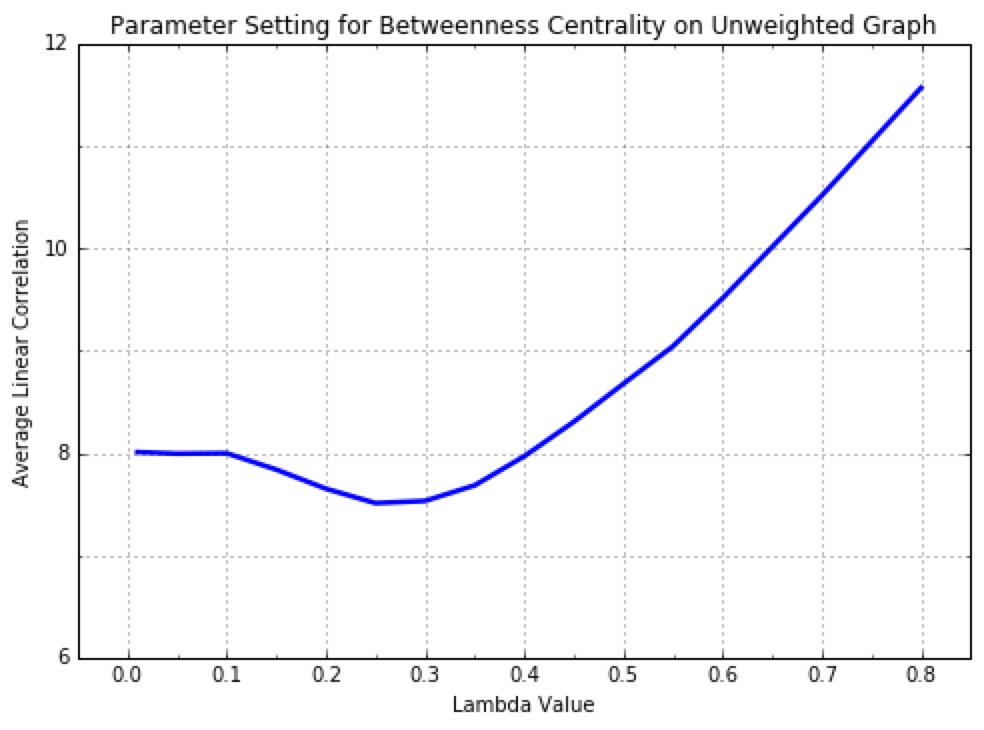
\includegraphics[width=0.95\linewidth]{BCU_2.jpeg}
%  \caption{Per-map suboptimality}
%  \label{acpermap}
\end{subfigure}
%\caption{Normalized mean suboptimality on the per-map and uni-map bases for GBDT, SVM, and NN classifiers using AlexNet as a feature extractor}
\begin{subfigure}{.4\textwidth}
	\centering
    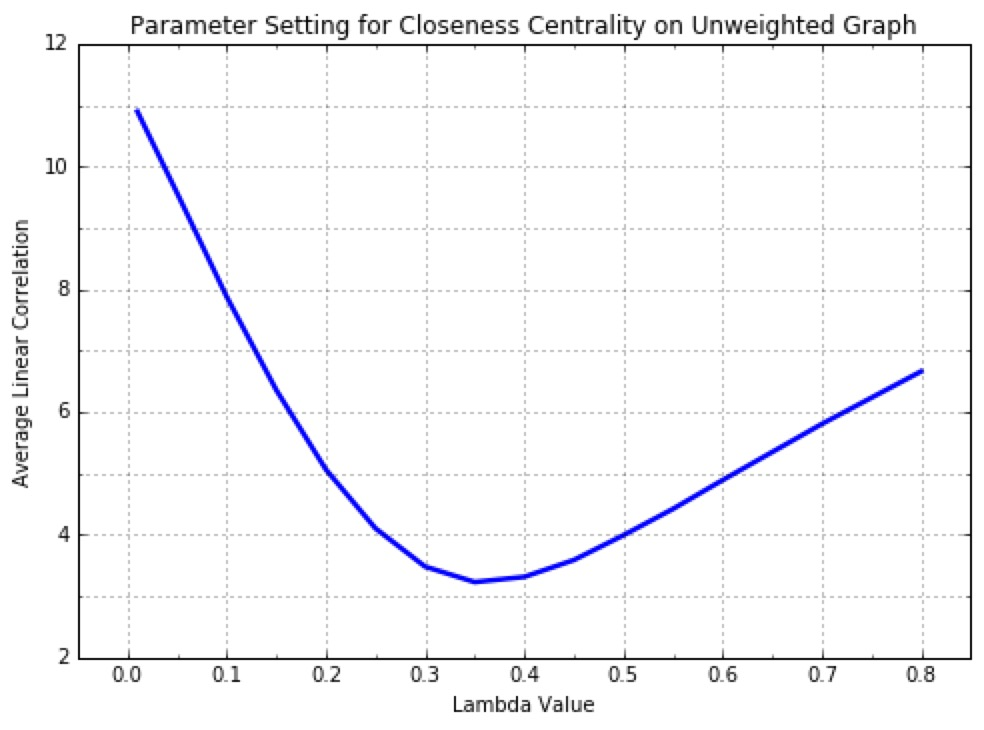
\includegraphics[width=0.95\linewidth]{CCU_2.jpeg}
\end{subfigure}

%\caption{Comparison of betweenness centralities computed by different methods on simulated weighted graphs}

\vspace{-0.1in}

\centering
\begin{subfigure}{.4\textwidth}
  \centering
  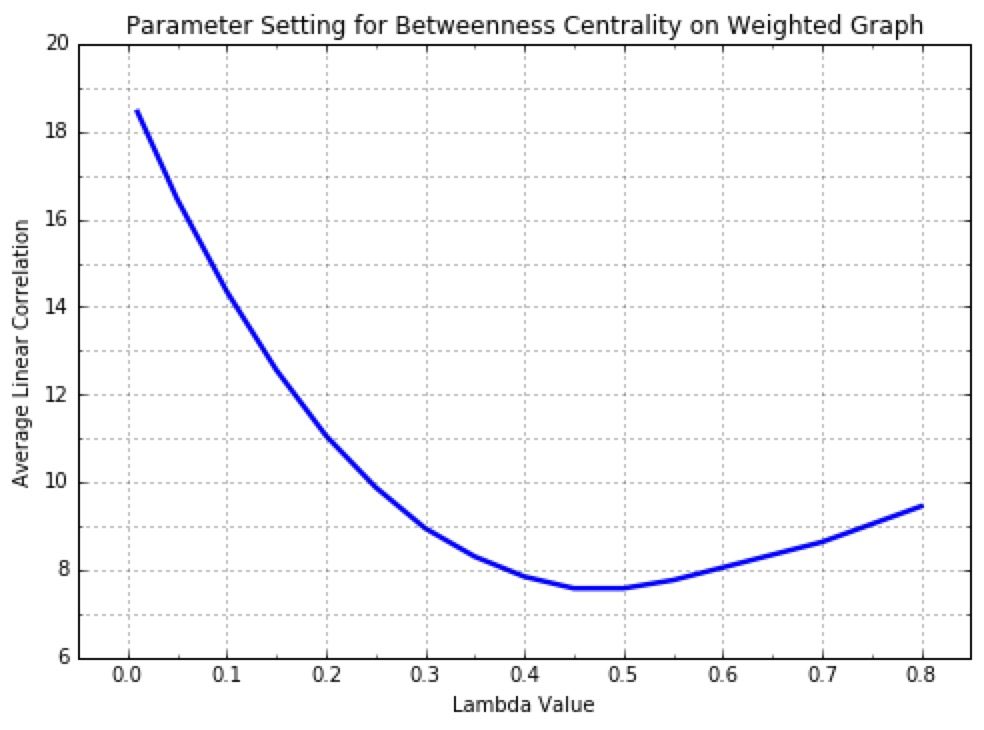
\includegraphics[width=0.95\linewidth]{BCW_2.jpeg}
%  \caption{Per-map suboptimality}
%  \label{acpermap}
\end{subfigure}
%\caption{Normalized mean suboptimality on the per-map and uni-map bases for GBDT, SVM, and NN classifiers using AlexNet as a feature extractor}
\begin{subfigure}{.4\textwidth}
	\centering
    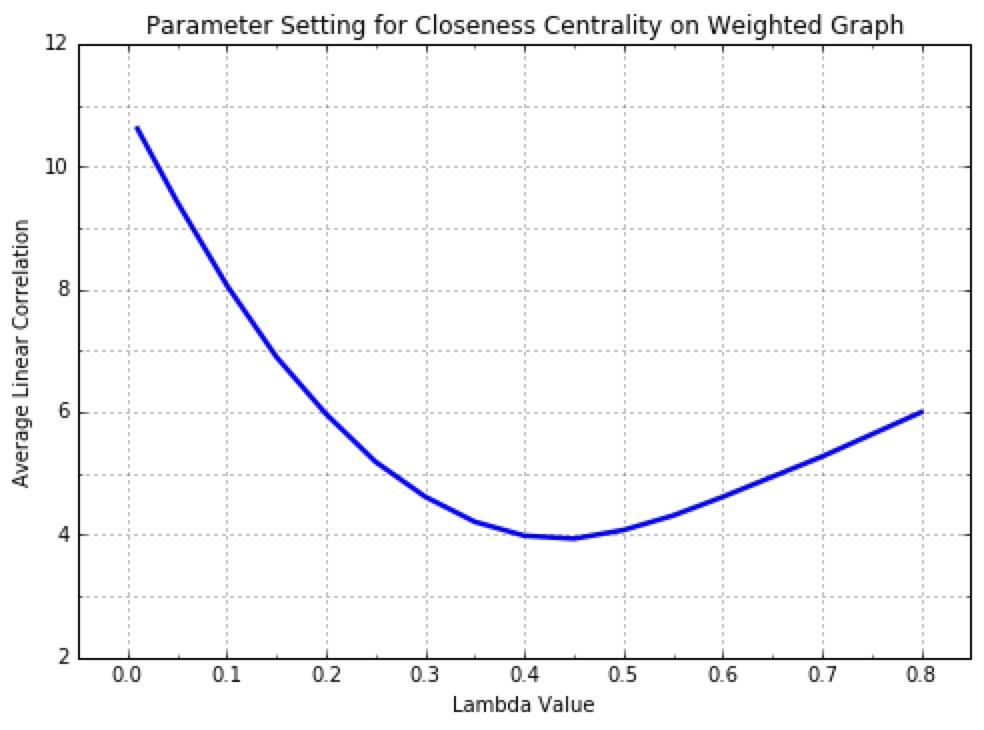
\includegraphics[width=0.95\linewidth]{CCW_2.jpeg}
\end{subfigure}
\caption{Hyper-parameter validation}
\end{figure}
%\caption{Betweenness Centrality on Enron Dataset}
\end{frame}



\section{Summary and Future Direction}
\begin{frame}
\frametitle{Summary}
\begin{itemize}
\item In this project we investigated the problem of calculating shortest path and centralities in the presence of edge uncertainty
\item We demonstrated the inability of taking the negative logarithm of edge probability as new edge weight
\item Based on the method of \textit{Most Probable Path}, we proposed a new and more direct way of computing shortest path and centralities of a graph, \textbf{Inversed Probabilistic Graph}
\item We empirically showed that under multiple circumstances, our approach outperforms previous approaches on related applications
\end{itemize}
\end{frame}

\begin{frame}
\frametitle{Future Direction}
Future directions can include research on
\begin{itemize}
\item How to detect community in the presence of edge uncertainty.
\end{itemize}
\end{frame}



%%%%%%%%%%%%%%%%%%%%%%%%%%%%%%%%%%%%%%%%%%%%%%%%%%%%%%%%%%%%%%%%%

% \begin{frame}{Font feature test}
%   \begin{itemize}
%     \item Regular
%     \item \textit{Italic}
%     \item \textsc{SmallCaps}
%     \item \textbf{Bold}
%     \item \textbf{\textit{Bold Italic}}
%     \item \textbf{\textsc{Bold SmallCaps}}
%     \item \texttt{Monospace}
%     \item \texttt{\textit{Monospace Italic}}
%     \item \texttt{\textbf{Monospace Bold}}
%     \item \texttt{\textbf{\textit{Monospace Bold Italic}}}
%   \end{itemize}
% \end{frame}

% \begin{frame}{Lists}
%   \begin{columns}[T,onlytextwidth]
%     \column{0.33\textwidth}
%       Items
%       \begin{itemize}
%         \item Milk \item Eggs \item Potatos
%       \end{itemize}

%     \column{0.33\textwidth}
%       Enumerations
%       \begin{enumerate}
%         \item First, \item Second and \item Last.
%       \end{enumerate}

%     \column{0.33\textwidth}
%       Descriptions
%       \begin{description}
%         \item[PowerPoint] Meeh. \item[Beamer] Yeeeha.
%       \end{description}
%   \end{columns}
% \end{frame}
% \begin{frame}{Animation}
%   \begin{itemize}[<+- | alert@+>]
%     \item \alert<4>{This is\only<4>{ really} important}
%     \item Now this
%     \item And now this
%   \end{itemize}
% \end{frame}
% \begin{frame}{Figures}
%   \begin{figure}
%     \newcounter{density}
%     \setcounter{density}{20}
%     \begin{tikzpicture}
%       \def\couleur{alerted text.fg}
%       \path[coordinate] (0,0)  coordinate(A)
%                   ++( 90:5cm) coordinate(B)
%                   ++(0:5cm) coordinate(C)
%                   ++(-90:5cm) coordinate(D);
%       \draw[fill=\couleur!\thedensity] (A) -- (B) -- (C) --(D) -- cycle;
%       \foreach \x in {1,...,40}{%
%           \pgfmathsetcounter{density}{\thedensity+20}
%           \setcounter{density}{\thedensity}
%           \path[coordinate] coordinate(X) at (A){};
%           \path[coordinate] (A) -- (B) coordinate[pos=.10](A)
%                               -- (C) coordinate[pos=.10](B)
%                               -- (D) coordinate[pos=.10](C)
%                               -- (X) coordinate[pos=.10](D);
%           \draw[fill=\couleur!\thedensity] (A)--(B)--(C)-- (D) -- cycle;
%       }
%     \end{tikzpicture}
%     \caption{Rotated square from
%     \href{http://www.texample.net/tikz/examples/rotated-polygons/}{texample.net}.}
%   \end{figure}
% \end{frame}
% \begin{frame}{Tables}
%   \begin{table}
%     \caption{Largest cities in the world (source: Wikipedia)}
%     \begin{tabular}{lr}
%       \toprule
%       City & Population\\
%       \midrule
%       Mexico City & 20,116,842\\
%       Shanghai & 19,210,000\\
%       Peking & 15,796,450\\
%       Istanbul & 14,160,467\\
%       \bottomrule
%     \end{tabular}
%   \end{table}
% \end{frame}
% \begin{frame}{Blocks}
%   Three different block environments are pre-defined and may be styled with an
%   optional background color.

%   \begin{columns}[T,onlytextwidth]
%     \column{0.5\textwidth}
%       \begin{block}{Default}
%         Block content.
%       \end{block}

%       \begin{alertblock}{Alert}
%         Block content.
%       \end{alertblock}

%       \begin{exampleblock}{Example}
%         Block content.
%       \end{exampleblock}

%     \column{0.5\textwidth}

%       \metroset{block=fill}

%       \begin{block}{Default}
%         Block content.
%       \end{block}

%       \begin{alertblock}{Alert}
%         Block content.
%       \end{alertblock}

%       \begin{exampleblock}{Example}
%         Block content.
%       \end{exampleblock}

%   \end{columns}
% \end{frame}
% \begin{frame}{Math}
%   \begin{equation*}
%     e = \lim_{n\to \infty} \left(1 + \frac{1}{n}\right)^n
%   \end{equation*}
% \end{frame}
% \begin{frame}{Line plots}
%   \begin{figure}
%     \begin{tikzpicture}
%       \begin{axis}[
%         mlineplot,
%         width=0.9\textwidth,
%         height=6cm,
%       ]

%         \addplot {sin(deg(x))};
%         \addplot+[samples=100] {sin(deg(2*x))};

%       \end{axis}
%     \end{tikzpicture}
%   \end{figure}
% \end{frame}
% \begin{frame}{Bar charts}
%   \begin{figure}
%     \begin{tikzpicture}
%       \begin{axis}[
%         mbarplot,
%         xlabel={Foo},
%         ylabel={Bar},
%         width=0.9\textwidth,
%         height=6cm,
%       ]

%       \addplot plot coordinates {(1, 20) (2, 25) (3, 22.4) (4, 12.4)};
%       \addplot plot coordinates {(1, 18) (2, 24) (3, 23.5) (4, 13.2)};
%       \addplot plot coordinates {(1, 10) (2, 19) (3, 25) (4, 15.2)};

%       \legend{lorem, ipsum, dolor}

%       \end{axis}
%     \end{tikzpicture}
%   \end{figure}
% \end{frame}
% \begin{frame}{Quotes}
%   \begin{quote}
%     Veni, Vidi, Vici
%   \end{quote}
% \end{frame}

% {%
% \setbeamertemplate{frame footer}{My custom footer}
% \begin{frame}[fragile]{Frame footer}
%     \themename defines a custom beamer template to add a text to the footer. It can be set via
%     \begin{verbatim}\setbeamertemplate{frame footer}{My custom footer}\end{verbatim}
% \end{frame}
% }

\begin{frame}{References}
\bibliography{demo}
\bibliographystyle{unsrt}
\end{frame}



% \begin{frame}{Summary}

%   Get the source of this theme and the demo presentation from

%   \begin{center}\url{github.com/matze/mtheme}\end{center}

%   The theme \emph{itself} is licensed under a
%   \href{http://creativecommons.org/licenses/by-sa/4.0/}{Creative Commons
%   Attribution-ShareAlike 4.0 International License}.

%   \begin{center}\ccbysa\end{center}

% \end{frame}

\begin{frame}[standout]
  Questions?
\end{frame}

% \appendix

% \begin{frame}[fragile]{Backup slides}
%   Sometimes, it is useful to add slides at the end of your presentation to
%   refer to during audience questions.

%   The best way to do this is to include the \verb|appendixnumberbeamer|
%   package in your preamble and call \verb|\appendix| before your backup slides.

%   \themename will automatically turn off slide numbering and progress bars for
%   slides in the appendix.
% \end{frame}

% \begin{frame}[allowframebreaks]{References}

%   \bibliography{demo}
%   \bibliographystyle{abbrv}

% \end{frame}

\end{document}
